%==============================================================
%  EE201 -- Circuit Theory I
%  Lecture 11 : Node Voltage Analysis -- slides
%  M. Mert Ankaralı, METU EEE
%
%  Compile:  ./build.sh      (or: pdflatex EE201_Lecture_11_slides.tex, twice)
%  Same colour code as the handout:
%      charge = purple, current = blue, voltage = orange, power = green
%==============================================================
\documentclass[11pt,aspectratio=169]{beamer}

\usepackage[T1]{fontenc}
\usepackage[utf8]{inputenc}
\usepackage[english]{babel}
\usepackage{lmodern}
\usepackage{amsmath,amssymb}
\usepackage{booktabs}
\usepackage{array}
\usepackage{colortbl}
\usepackage{tikz}
\usepackage[american,siunitx]{circuitikz}
\usetikzlibrary{matrix,arrows.meta,positioning,calc,decorations.pathreplacing,decorations.pathmorphing,decorations.markings}
\usetikzlibrary{overlay-beamer-styles}

%-------------------- plain METU-flavoured theme --------------
\usetheme{default}
\usecolortheme{default}
\useinnertheme{rectangles}
\setbeamertemplate{navigation symbols}{}
\setbeamertemplate{itemize items}[square]
\setbeamerfont{frametitle}{size=\large,series=\bfseries}
\setbeamerfont{title}{size=\LARGE,series=\bfseries}

\definecolor{metured}{RGB}{155,27,48}
\definecolor{metugray}{RGB}{88,89,91}
\definecolor{metulight}{RGB}{243,240,241}
\definecolor{ccur}{RGB}{0,102,170}
\definecolor{cvolt}{RGB}{214,120,0}
\definecolor{cpow}{RGB}{23,128,74}
\definecolor{ccharge}{RGB}{124,60,160}
\definecolor{cflux}{RGB}{0,138,138}
\definecolor{copper}{RGB}{184,98,30}

\setbeamercolor{structure}{fg=metured}
\setbeamercolor{frametitle}{fg=metured,bg=}
\setbeamercolor{title}{fg=metured}
\setbeamercolor{normal text}{fg=black!88}
\setbeamercolor{block title}{fg=white,bg=metured}
\setbeamercolor{block body}{bg=metulight}
\setbeamercolor{alerted text}{fg=metured}

\setbeamertemplate{frametitle}{%
  \vspace{0.55em}%
  \usebeamerfont{frametitle}\usebeamercolor[fg]{frametitle}\insertframetitle\par
  \vspace{-0.2em}{\color{metured}\rule{\textwidth}{1pt}}\par\vspace{-0.2em}}

\setbeamertemplate{footline}{%
  \hbox{\begin{beamercolorbox}[wd=\paperwidth,ht=2.4ex,dp=1.4ex,leftskip=1.2em,rightskip=1.2em]{}%
  \tiny\color{metugray}\coursecode\ \textbar\ Lecture 11: Node Voltage Analysis
  \hfill \insertframenumber/\inserttotalframenumber
  \end{beamercolorbox}}}

%-------------------- macros ----------------------------------
\newcommand{\coursecode}{EE201}
\newcommand{\term}{Fall 2026--2027}
\newcommand{\Icol}[1]{\textcolor{ccur}{#1}}
\newcommand{\Vcol}[1]{\textcolor{cvolt}{#1}}
\newcommand{\Pcol}[1]{\textcolor{cpow}{#1}}
\newcommand{\Qcol}[1]{\textcolor{ccharge}{#1}}
\newcommand{\Fcol}[1]{\textcolor{cflux}{#1}}
\newcommand{\uni}[1]{\,\mathrm{#1}}
\newcommand{\A}{\uni{A}} \newcommand{\V}{\uni{V}}
\newcommand{\W}{\uni{W}} \newcommand{\J}{\uni{J}}
\newcommand{\Cb}{\uni{C}} \newcommand{\s}{\uni{s}}
\newcommand{\Wb}{\uni{Wb}} \newcommand{\Hy}{\uni{H}}
\newcommand{\Sie}{\uni{S}}


%  voltage sources: smaller + and - inside the circle, further apart
\ctikzset{bipoles/vsourceam/inner plus={\tiny$+$},
          bipoles/vsourceam/inner minus={\tiny$\vphantom{+}-$},
          bipoles/vsourceam/margin=0.85,
          bipoles/cvsourceam/inner plus={\tiny$+$},
          bipoles/cvsourceam/inner minus={\tiny$\vphantom{+}-$},
          bipoles/cvsourceam/margin=0.85}
\ctikzset{bipoles/length=0.9cm, label/align=straight,
          bipoles/generic/height=0.28, bipoles/generic/width=0.62}
\tikzset{
  iar/.style={-{Stealth[length=2.2mm]}, ccur, thick},
  glab/.style={font=\footnotesize, text=metured},
  ttl/.style={font=\scriptsize\bfseries, text=metugray},
  capn/.style={font=\scriptsize, text=metugray, align=center},
  pol/.style={font=\small, text=cvolt},
  nlab/.style={circle, draw=metured, text=metured, font=\scriptsize, inner sep=0.7pt},
  blab/.style={font=\footnotesize, text=black!80},
  gbr/.style={black!75, thick, postaction={decorate, decoration={markings,
      mark=at position 0.56 with {\arrow{Stealth[length=2.5mm]}}}}},
  hal/.style={draw=cpow!60, line width=6pt, opacity=0.35, line cap=round, line join=round},
  halo/.style={circle, fill=metured!16, minimum size=0.95cm},
  elem/.style={draw=metugray, thick, fill=metulight},
  bigarr/.style={-{Stealth[length=3mm]}, very thick, metugray},
}

%-------------------- Lecture 11 circuit macros ---------------
\newcommand{\ohm}{\,\Omega}
\newcommand{\e}[1]{\textcolor{cvolt}{e_{#1}}}
\newcommand{\ep}[1]{\textcolor{cvolt}{e_{#1}'}}
\newcommand{\nd}[1]{\tikz[baseline=(c.base)]\node[nlab](c){#1};}
\newcommand{\vbf}[1]{\textcolor{cvolt}{\mathbf{#1}}}
\newcommand{\ibf}[1]{\textcolor{ccur}{\mathbf{#1}}}
%  A node: dot at (#1) with label #3 placed at anchor #2
\newcommand{\nodev}[3]{\fill (#1) circle (1.7pt) node[#2, inner sep=2pt, font=\small, text=cvolt] {#3};}
%  Ground symbol below (#1,0)
\newcommand{\gnd}[1]{\draw (#1,0) -- (#1,-0.2) node[ground] {};}
%  Examples 11.1 and 11.2.
%  #1 = 0: i_s1, R1..R5, i_s2 (11.1);  1: i_s, R1..R4, v_s to ground (11.2);
%  2: as 1, e_3 not a label (11.2 revisited)
\newcommand{\exA}[1]{%
  \ifnum#1=0
    \draw (0,0) to[american current source, l=$\Icol{i_{s1}}$] (0,2);
  \else
    \draw (0,0) to[american current source, l=$\Icol{i_s}$] (0,2);
  \fi
  \draw (0,2) -- (1.8,2) to[R, l=$R_2$] (3.8,2) to[R, l_=$R_4$] (5.8,2);
  \draw (1.8,2) to[R, l_=$R_1$] (1.8,0);
  \draw (3.8,2) to[R, l_=$R_3$] (3.8,0);
  \draw (0,0) -- (5.8,0);
  \ifnum#1=0
    \draw (3.8,2) -- (3.8,3.0) to[R, l=$R_5$] (5.8,3.0) -- (5.8,2);
    \draw (5.8,2) to[american current source, l=$\Icol{i_{s2}}$] (5.8,0);
    \nodev{3.8,2}{above left}{$e_2$}
    \nodev{5.8,2}{above right}{$e_3$}
  \else
    \draw (5.8,0) to[american voltage source, invert, l_=$\Vcol{v_s}$] (5.8,2);
    \nodev{3.8,2}{above}{$e_2$}
    \ifnum#1=1 \nodev{5.8,2}{above}{$e_3$}\else \fill (5.8,2) circle (1.7pt);\fi
  \fi
  \nodev{1.8,2}{above}{$e_1$}
  \gnd{3.8}}
%  Example 11.3: two voltage sources; v_s2 between nodes 1 and 2.
%  #1 = 0: plain;  1: current i through v_s2;  2: the supernode
\newcommand{\exB}[1]{%
  \draw (0,0) to[american voltage source, invert, l=$\Vcol{v_{s1}}$] (0,2);
  \draw (0,2) to[R, l=$R_1$] (1.8,2) to[american voltage source, l=$\Vcol{v_{s2}}$] (3.6,2)
        to[R, l=$R_4$] (5.4,2) -- (7.0,2);
  \draw (1.8,2) to[R, l=$R_2$] (1.8,0);
  \draw (3.6,2) to[R, l=$R_3$] (3.6,0);
  \draw (5.4,0) to[american current source, l_=$\Icol{i_{s1}}$] (5.4,2);
  \draw (7.0,2) to[R, l=$R_5$] (7.0,0);
  \draw (0,0) -- (7.0,0);
  \nodev{1.8,2}{above right}{$e_1$}
  \nodev{3.6,2}{above left}{$e_2$}
  \nodev{5.4,2}{above}{$e_3$}
  \ifnum#1=1
    \draw[iar] (2.55,1.5) -- (3.05,1.5);
    \node[font=\small, text=ccur] at (2.8,1.25) {$i$};
  \fi
  \ifnum#1=2
    \draw[dashed, metured, thick, rounded corners=4pt] (1.5,1.6) rectangle (3.9,2.95);
    \node[font=\scriptsize, text=metured, anchor=south] at (2.7,2.95) {supernode};
  \fi
  \gnd{1.8}}
%  Example 11.4: a dependent voltage source v_x between nodes 3 and 2.
%  #1 = 0: plain;  1: the supernode S;  2: node 3 as the ground
\newcommand{\exC}[1]{%
  \draw (0,0) to[american current source, l=$5\A$] (0,2) -- (0,3.4)
        to[R, l=$2\ohm$] (1.8,3.4)
        to[american controlled voltage source, invert, l=$\Vcol{v_x}$] (4.2,3.4) -- (4.2,2);
  \draw (0,2) -- (2.2,2) to[R, l=$2\ohm$] (4.2,2);
  \draw (2.2,2) to[R, l=$4\ohm$] (2.2,0);
  \draw (4.2,2) to[R, l=$3\ohm$] (4.2,0);
  \draw (0,0) -- (4.2,0);
  \fill (0,2) circle (1.7pt);
  \node[pol] at (1.82,1.55) {$+$}; \node[pol] at (1.82,0.45) {$-$};
  \node[font=\small, text=cvolt] at (1.5,1.0) {$v_x$};
  \ifnum#1=2
    \nodev{2.2,2}{above right}{$e_1'$}
    \nodev{4.2,2}{right}{$e_2'$}
    \fill (1.8,3.4) circle (1.7pt);
    \draw (1.8,3.4) -- (1.8,3.1) node[ground] {};
    \nodev{2.2,0}{below}{$e_0'$}
  \else
    \nodev{2.2,2}{above right}{$e_1$}
    \nodev{4.2,2}{right}{$e_2$}
    \nodev{1.8,3.4}{above right}{$e_3$}
    \gnd{2.2}
  \fi
  \ifnum#1=1
    \draw[dashed, metured, thick, rounded corners=4pt]
      (1.55,4.45) -- (4.95,4.45) -- (4.95,1.6) -- (3.85,1.6) -- (3.85,2.9) -- (1.55,2.9) -- cycle;
    \node[nlab] at (5.25,4.45) {S};
  \fi}
%  A first small example: i_s, R1, R2, R3.  #1 = 0: branch voltages and currents only;
%  1: also the ground and the node voltages
\newcommand{\exI}[1]{%
  \draw (0,0) to[american current source, l=$\Icol{i_s}$] (0,2.6) -- (2.4,2.6)
        to[R, l=$R_2$] (5.2,2.6);
  \draw (2.4,2.6) to[R, l=$R_1$] (2.4,0);
  \draw (5.2,2.6) to[R, l=$R_3$] (5.2,0);
  \draw (0,0) -- (5.2,0);
  \node[pol] at (2.05,1.75) {$+$}; \node[pol] at (2.05,0.85) {$-$};
  \node[font=\small, text=cvolt] at (1.75,1.3) {$v_1$};
  \node[pol] at (3.42,2.25) {$+$}; \node[pol] at (4.25,2.25) {$-$};
  \node[font=\small, text=cvolt] at (3.8,2.22) {$v_2$};
  \node[pol] at (4.85,1.75) {$+$}; \node[pol] at (4.85,0.85) {$-$};
  \node[font=\small, text=cvolt] at (4.55,1.3) {$v_3$};
  \draw[iar] (2.62,2.45) -- (2.62,2.0); \node[font=\small, text=ccur] at (2.88,2.22) {$i_1$};
  \draw[iar] (2.65,2.85) -- (3.1,2.85); \node[font=\small, text=ccur] at (2.88,3.12) {$i_2$};
  \draw[iar] (5.42,2.45) -- (5.42,2.0); \node[font=\small, text=ccur] at (5.68,2.22) {$i_3$};
  \ifnum#1=1
    \nodev{2.4,2.6}{above left}{$e_1$}
    \nodev{5.2,2.6}{above}{$e_2$}
    \gnd{3.8}
  \fi}
\newcommand{\yes}{\textcolor{cpow}{\checkmark}}
\newcommand{\no}{\textcolor{metured}{$\boldsymbol{\times}$}}
\hypersetup{colorlinks=true,allcolors=metured}
\tikzset{fbox/.style={draw=metugray, thick, fill=metulight, rounded corners=3pt,
                      minimum height=0.9cm, align=center, font=\small, inner sep=4pt}}

\title{Lecture 11: Node Voltage Analysis}
\subtitle{EE201 -- Circuit Theory I}
\author{M. Mert Ankaralı}
\institute{\small Department of Electrical and Electronics Engineering\\
           Middle East Technical University}
\date{}

%  Roadmap of the lecture; #1 = current part (1-7)
\newcommand{\rmitem}[2]{%
  \item \ifnum#1<\rmcur\relax \textcolor{black!35}{#2}\ \textcolor{cpow}{\checkmark}%
        \else\ifnum#1=\rmcur\relax \textcolor{metured}{\textbf{#2}}%
        \else #2\fi\fi}
\newcommand{\roadmapframe}[1]{%
  \begin{frame}{Roadmap}
    \def\rmcur{#1}%
    \vfill
    \begin{enumerate}\itemsep8pt
      \rmitem{1}{The idea of node voltage analysis}
      \rmitem{2}{Resistors and current sources}
      \rmitem{3}{A voltage source connected to the ground}
      \rmitem{4}{A voltage source between two nodes: Method I}
      \rmitem{5}{A voltage source between two nodes: Method II, the supernode}
      \rmitem{6}{Dependent sources}
      \rmitem{7}{Choosing the ground}
    \end{enumerate}
    \vfill
  \end{frame}}


%  The chain built up over the three steps: #1 = number of boxes (2-4)
\newcommand{\chain}[1]{%
  \begin{tikzpicture}[node distance=1.7cm, every node/.style={font=\small},
                      fbox/.append style={minimum width=1.9cm, font=\scriptsize}]
    \node[fbox] (e) {$\Vcol{\mathbf{e}}$\\[-2pt]{\scriptsize node voltages}};
    \node[fbox, right=of e] (v) {$\Vcol{\mathbf{v}}$\\[-2pt]{\scriptsize branch voltages}};
    \draw[bigarr] (e) -- node[above, font=\scriptsize, text=black] {KVL holds} (v);
    \ifnum#1>2
      \node[fbox, right=of v] (i) {$\Icol{\mathbf{i}}$\\[-2pt]{\scriptsize branch currents}};
      \draw[bigarr] (v) -- node[above, font=\scriptsize, text=black] {Ohm's law} (i);
    \fi
    \ifnum#1>3
      \node[fbox, right=of i, draw=metured, fill=metured!8] (k) {$n-1$ equations\\[-2pt]{\scriptsize in $\Vcol{\mathbf{e}}$}};
      \draw[bigarr] (i) -- node[above, font=\scriptsize, text=black] {KCL} (k);
    \fi
  \end{tikzpicture}}

\begin{document}

%--------------------------------------------------------------
\begin{frame}[plain]
  \titlepage
  \vspace{-1.2em}
  \begin{center}\scriptsize\color{metugray}
    \Icol{$\blacksquare$}~current \quad \Vcol{$\blacksquare$}~voltage, node voltage $e$ \quad
    \textcolor{metured}{$\blacksquare$}~supernode
  \end{center}
\end{frame}

%--------------------------------------------------------------
\begin{frame}{Review: two ways to solve an LTI resistive circuit}
  \begin{columns}[t,onlytextwidth]
    \begin{column}{0.47\textwidth}
      \begin{block}{Transform the circuit}
        \begin{itemize}\itemsep3pt
          \item Substitution, equivalent one-ports.
          \item Series and parallel connections.
          \item Source transformation.
        \end{itemize}
        \vspace{3pt}
        Works for \alert{many} circuits, but not all.
      \end{block}
    \end{column}
    \begin{column}{0.47\textwidth}
      \begin{block}{Write its equations as it is}
        \begin{itemize}\itemsep3pt
          \item KCL: $A\Icol{\mathbf{i}} = \mathbf{0}$.
          \item KVL: $\Vcol{\mathbf{v}} = A^T\Vcol{\mathbf{e}}$.
          \item One element law per branch.
        \end{itemize}
        \vspace{3pt}
        Works for \alert{every} circuit.
      \end{block}
    \end{column}
  \end{columns}
  \vfill
  \begin{center}
    With the node voltages $\Vcol{\mathbf{e}}$ as the unknowns, KVL holds
    \alert{automatically}.\\[4pt]
    Only KCL is left to write.
  \end{center}
  \vfill
\end{frame}

%--------------------------------------------------------------
\begin{frame}{Motivation}
  \vfill
  \begin{itemize}\itemsep10pt
    \item So far, we solved circuits by simplifying them: series, parallel, source
      transformation.
    \item<2-> These simplifications do \alert{not} work for every circuit.
    \item<3-> \alert{Node voltage analysis} writes the equations of the circuit directly,
      without changing the circuit.
    \item<4-> Its unknowns are only the $n - 1$ \alert{node voltages}, instead of $2b$ branch
      voltages and currents.
    \item<5-> Its steps are the same for \alert{every} LTI resistive circuit.
    \item<6-> Later, \alert{mesh current analysis} will do the same with mesh currents.
  \end{itemize}
  \vfill
\end{frame}

%==============================================================
\roadmapframe{1}

%--------------------------------------------------------------
\begin{frame}{The idea: a small example}
  \begin{columns}[c,onlytextwidth]
    \begin{column}{0.5\textwidth}
      \centering
      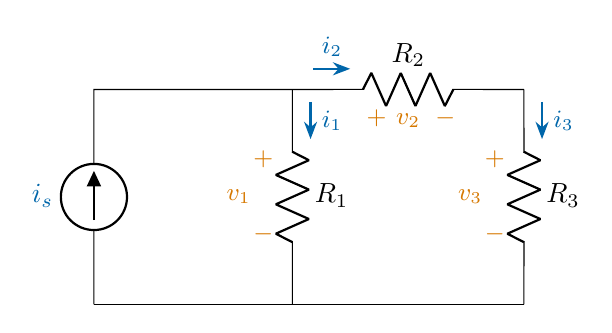
\begin{tikzpicture}[scale=1.05]
        \exI{0}
      \end{tikzpicture}
    \end{column}
    \begin{column}{0.47\textwidth}
      \textbf{Question.} How many unknowns does this circuit have?\\[12pt]
      \onslide<2->{%
      $4$ branches: $4$ branch voltages and $4$ branch currents.\\[8pt]}
      \onslide<3->{%
      So $8$ unknowns, and we would need $8$ equations.\\[12pt]}
      \onslide<4->{%
      With node voltages, only \alert{2} unknowns are left.\\[4pt]
      Three steps show how.}
    \end{column}
  \end{columns}
\end{frame}

%--------------------------------------------------------------
\begin{frame}{Step 1: node voltages give the branch voltages}
  \begin{columns}[c,onlytextwidth]
    \begin{column}{0.5\textwidth}
      \centering
      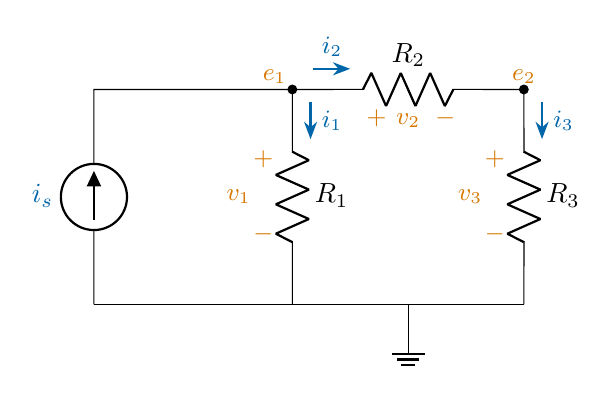
\begin{tikzpicture}[scale=1.05]
        \exI{1}
      \end{tikzpicture}
    \end{column}
    \begin{column}{0.47\textwidth}
      Choose the bottom node as the ground.\\[3pt]
      Call the other node voltages $\e{1}$ and $\e{2}$.\\[10pt]
      \onslide<2->{%
      $\Vcol{v_1} = \e{1}, \qquad \Vcol{v_2} = \e{1} - \e{2}, \qquad \Vcol{v_3} = \e{2}$\\[10pt]}
      \onslide<3->{%
      \textbf{Question.} Does KVL hold around the loop $R_1$, $R_2$, $R_3$?\\[6pt]}
      \onslide<4->{%
      $\Vcol{v_1} = \Vcol{v_2} + \Vcol{v_3}$: \ $\e{1} = (\e{1} - \e{2}) + \e{2}$ \ \yes\\[4pt]
      KVL holds \alert{automatically}, for any $\e{1}$, $\e{2}$.}
    \end{column}
  \end{columns}
  \vfill
  \onslide<4->{\begin{center}\chain{2}\end{center}}
\end{frame}

%--------------------------------------------------------------
\begin{frame}{Step 2: the element laws give the branch currents}
  \begin{columns}[c,onlytextwidth]
    \begin{column}{0.5\textwidth}
      \centering
      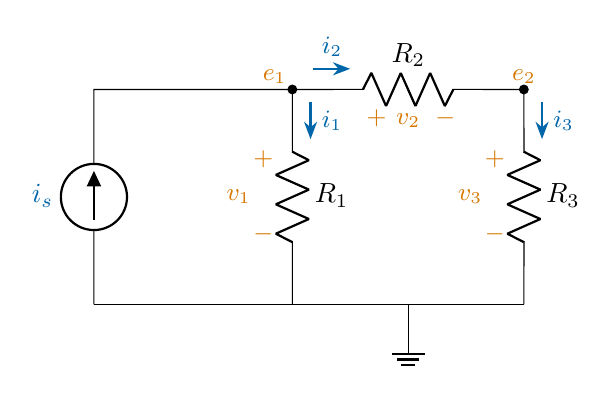
\begin{tikzpicture}[scale=1.05]
        \exI{1}
      \end{tikzpicture}
    \end{column}
    \begin{column}{0.47\textwidth}
      Each resistor obeys $\Icol{i} = \Vcol{v}/R$:\\[10pt]
      \onslide<2->{%
      $\displaystyle \Icol{i_1} = \frac{\e{1}}{R_1}, \qquad
       \Icol{i_2} = \frac{\e{1} - \e{2}}{R_2}, \qquad
       \Icol{i_3} = \frac{\e{2}}{R_3}$\\[10pt]}
      \onslide<3->{%
      Every branch current is now written with $\e{1}$ and $\e{2}$.}
    \end{column}
  \end{columns}
  \vfill
  \begin{center}\chain{3}\end{center}
\end{frame}

%--------------------------------------------------------------
\begin{frame}{Step 3: KCL gives the equations}
  \begin{columns}[c,onlytextwidth]
    \begin{column}{0.5\textwidth}
      \centering
      \begin{tikzpicture}[scale=1.05]
        \only<1>{\node[halo] at (2.4,2.6) {};}
        \only<2>{\node[halo] at (5.2,2.6) {};}
        \exI{1}
      \end{tikzpicture}
    \end{column}
    \begin{column}{0.47\textwidth}
      \textbf{Node 1:} \
      $\displaystyle -\Icol{i_s} + \frac{\e{1}}{R_1} + \frac{\e{1} - \e{2}}{R_2} = 0$\\[10pt]
      \onslide<2->{%
      \textbf{Node 2:} \
      $\displaystyle -\frac{\e{1} - \e{2}}{R_2} + \frac{\e{2}}{R_3} = 0$\\[12pt]}
      \onslide<3->{%
      Two equations, two unknowns: solve for $\e{1}$ and $\e{2}$.\\[6pt]}
      \onslide<4->{%
      Then Steps 1 and 2 give all branch voltages and currents.}
    \end{column}
  \end{columns}
  \vfill
  \onslide<3->{\begin{center}\chain{4}\end{center}}
\end{frame}

%--------------------------------------------------------------
\begin{frame}{The procedure}
  \begin{columns}[c,onlytextwidth]
    \begin{column}{0.52\textwidth}
      \begin{enumerate}\itemsep10pt
        \item Choose a \alert{reference node} (ground); its node voltage is $0$.
        \item<2-> Label the other node voltages $\e{1}, \dots, \e{n-1}$.
        \item<3-> Write \alert{KCL} at every other node, in terms of node voltages.
      \end{enumerate}
    \end{column}
    \begin{column}{0.44\textwidth}
      \centering
      \onslide<3->{%
      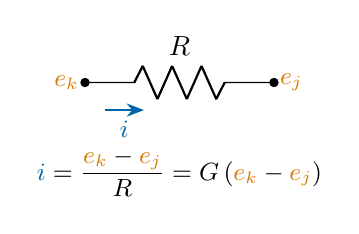
\begin{tikzpicture}
        \draw (0,1.6) to[R, l=$R$] (2.4,1.6);
        \nodev{0,1.6}{left}{$e_k$} \nodev{2.4,1.6}{right}{$e_j$}
        \draw[iar] (0.25,1.25) -- (0.75,1.25); \node[font=\small, text=ccur] at (0.5,1.0) {$i$};
        \node[font=\small] at (1.2,0.45)
          {$\Icol{i} = \dfrac{\e{k} - \e{j}}{R} = G\,(\e{k} - \e{j})$};
      \end{tikzpicture}\\[10pt]}
      \onslide<4->{%
      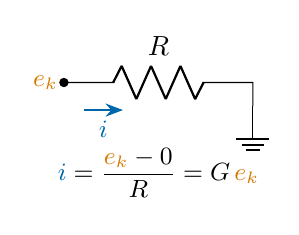
\begin{tikzpicture}
        \draw (0,1.6) to[R, l=$R$] (2.4,1.6) -- (2.4,1.3) node[ground] {};
        \nodev{0,1.6}{left}{$e_k$}
        \draw[iar] (0.25,1.25) -- (0.75,1.25); \node[font=\small, text=ccur] at (0.5,1.0) {$i$};
        \node[font=\small] at (1.2,0.45) {$\Icol{i} = \dfrac{\e{k} - 0}{R} = G\,\e{k}$};
      \end{tikzpicture}}
    \end{column}
  \end{columns}
  \vfill
  \onslide<5->{\begin{center}
    The current \alert{leaving} node $k$ through a resistor is its own node voltage minus the
    other one, over $R$.
  \end{center}}
\end{frame}

%==============================================================
\roadmapframe{2}

%--------------------------------------------------------------
\begin{frame}{Example 11.1: only current sources}
  \begin{columns}[c,onlytextwidth]
    \begin{column}{0.5\textwidth}
      \centering
      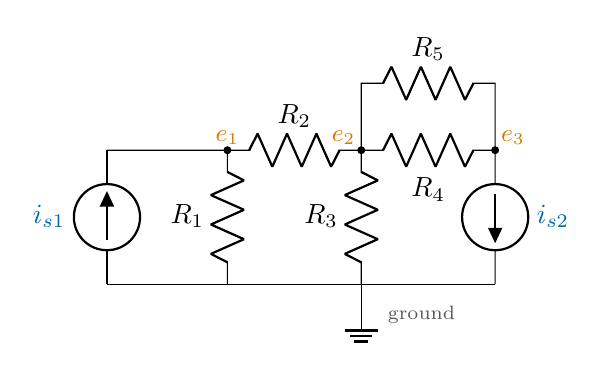
\begin{tikzpicture}[scale=0.85]
        \exA{0}
        \node[font=\scriptsize, text=metugray, anchor=west] at (4.05,-0.45) {ground};
      \end{tikzpicture}
    \end{column}
    \begin{column}{0.46\textwidth}
      \textbf{Question.} How many unknowns does this circuit have?\\[3pt]
      How many does node voltage analysis need?\\[12pt]
      \onslide<2->{%
      $b = 7$ branches: $2b = \alert{14}$ branch voltages and currents.\\[8pt]}
      \onslide<3->{%
      $n = 4$ nodes: only \alert{3} node voltages, $\e{1}$, $\e{2}$, $\e{3}$.\\[8pt]}
      \onslide<4->{%
      So we need three KCL equations, at nodes 1, 2 and 3.}
    \end{column}
  \end{columns}
\end{frame}

%--------------------------------------------------------------
\begin{frame}{Example 11.1: KCL at each node}
  \begin{columns}[c,onlytextwidth]
    \begin{column}{0.47\textwidth}
      \centering
      \begin{tikzpicture}[scale=0.8]
        \only<1>{\node[halo] at (1.8,2) {};}
        \only<2>{\node[halo] at (3.8,2) {};}
        \only<3>{\node[halo] at (5.8,2) {};}
        \exA{0}
      \end{tikzpicture}
    \end{column}
    \begin{column}{0.5\textwidth}
      \small
      \textbf{Node 1:}\\[2pt]
      $\displaystyle -\Icol{i_{s1}} + \frac{\e{1}}{R_1} + \frac{\e{1} - \e{2}}{R_2} = 0$\\[8pt]
      \onslide<2->{%
      \textbf{Node 2:}\\[2pt]
      $\displaystyle \frac{\e{2} - \e{1}}{R_2} + \frac{\e{2}}{R_3} + \frac{\e{2} - \e{3}}{R_4}
        + \frac{\e{2} - \e{3}}{R_5} = 0$\\[8pt]}
      \onslide<3->{%
      \textbf{Node 3:}\\[2pt]
      $\displaystyle \frac{\e{3} - \e{2}}{R_4} + \frac{\e{3} - \e{2}}{R_5} + \Icol{i_{s2}} = 0$\\[8pt]}
      \onslide<4->{%
      Every term is a current \alert{leaving} the node.\\[2pt]
      A source pointing \alert{into} the node enters with a minus sign.}
    \end{column}
  \end{columns}
\end{frame}

%--------------------------------------------------------------
\begin{frame}{Example 11.1: matrix form}
  \vfill
  With the conductances $G_k = 1/R_k$:
  \[
    \begin{aligned}
      (G_1 + G_2)\,\e{1} - G_2\,\e{2} &= \Icol{i_{s1}}\\
      -G_2\,\e{1} + (G_2 + G_3 + G_4 + G_5)\,\e{2} - (G_4 + G_5)\,\e{3} &= 0\\
      -(G_4 + G_5)\,\e{2} + (G_4 + G_5)\,\e{3} &= -\Icol{i_{s2}}
    \end{aligned}
  \]
  \vfill
  \onslide<2->{%
  \[
    \underbrace{\begin{bmatrix}
      G_1 + G_2 & -G_2 & 0\\
      -G_2 & G_2 + G_3 + G_4 + G_5 & -(G_4 + G_5)\\
      0 & -(G_4 + G_5) & G_4 + G_5
    \end{bmatrix}}_{Y_n}
    \underbrace{\begin{bmatrix} \e{1}\\ \e{2}\\ \e{3} \end{bmatrix}}_{\Vcol{\mathbf{e}}}
    =
    \underbrace{\begin{bmatrix} \Icol{i_{s1}}\\ 0\\ -\Icol{i_{s2}} \end{bmatrix}}_{\Icol{\mathbf{i}_s}}
  \]}
  \vfill
  \onslide<3->{\begin{center}
    $Y_n$ is the \alert{node admittance matrix}: \ $Y_n\Vcol{\mathbf{e}} = \Icol{\mathbf{i}_s}$.
  \end{center}}
  \vfill
\end{frame}

%--------------------------------------------------------------
\begin{frame}{Writing $Y_n$ by inspection}
  \begin{columns}[c,onlytextwidth]
    \begin{column}{0.48\textwidth}
      \centering
      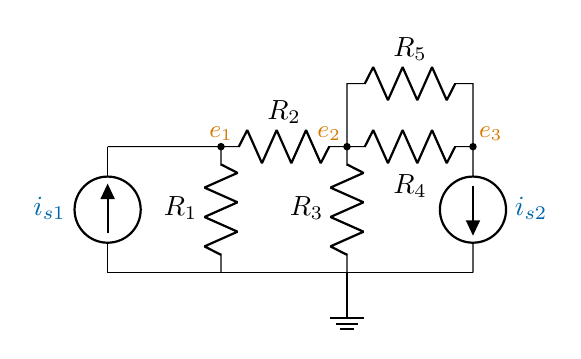
\begin{tikzpicture}[scale=0.8]
        \exA{0}
      \end{tikzpicture}\\[8pt]
      {\small
      $\begin{bmatrix}
        \alert{G_1 + G_2} & -G_2 & 0\\
        -G_2 & \alert{G_2 + \dots + G_5} & -(G_4 + G_5)\\
        0 & -(G_4 + G_5) & \alert{G_4 + G_5}
      \end{bmatrix}$}
    \end{column}
    \begin{column}{0.5\textwidth}
      \small
      \textbf{Question.} Can you read each entry of $Y_n$ directly from the circuit?\\[10pt]
      \onslide<2->{%
      \textbf{Diagonal} $(k,k)$: the sum of the conductances \alert{connected to} node $k$.\\[7pt]}
      \onslide<3->{%
      \textbf{Off-diagonal} $(k,j)$: minus the sum of the conductances \alert{between} nodes $k$
      and $j$.\\[7pt]}
      \onslide<4->{%
      \textbf{Right side} $k$: the sum of the source currents \alert{entering} node $k$.\\[7pt]}
      \onslide<5->{%
      So $Y_n$ is \alert{symmetric}: the entry $(k,j)$ equals the entry $(j,k)$.}
    \end{column}
  \end{columns}
\end{frame}

%--------------------------------------------------------------
\begin{frame}{Why is $Y_n$ symmetric?}
  \vfill
  Split $A$ into the resistor branches and the current source branches:
  $A = [\,A_R \ \ A_S\,]$.
  \vfill
  \begin{columns}[t,onlytextwidth]
    \begin{column}{0.5\textwidth}
      \begin{itemize}\itemsep6pt
        \item<2-> KCL: \ $A_R\Icol{\mathbf{i}_R} + A_S\Icol{\mathbf{i}_S} = \mathbf{0}$.
        \item<3-> Resistors: \ $\Icol{\mathbf{i}_R} = G\,\Vcol{\mathbf{v}_R}$, \
          $G = \mathrm{diag}(G_1, \dots, G_5)$.
        \item<4-> KVL: \ $\Vcol{\mathbf{v}_R} = A_R^T\Vcol{\mathbf{e}}$.
      \end{itemize}
    \end{column}
    \begin{column}{0.46\textwidth}
      \onslide<5->{%
      \[
        \underbrace{A_R\, G\, A_R^T}_{Y_n}\,\Vcol{\mathbf{e}} = \underbrace{-A_S\Icol{\mathbf{i}_S}}_{\Icol{\mathbf{i}_s}}
      \]}
      \onslide<6->{%
      \[
        Y_n^T = A_R\, G^T A_R^T = A_R\, G\, A_R^T = Y_n
      \]}
    \end{column}
  \end{columns}
  \vfill
  \onslide<7->{\begin{center}
    $G$ is diagonal, so $Y_n$ is symmetric.\\[3pt]
    $-A_S\Icol{\mathbf{i}_S}$ adds up the source currents entering each node.
  \end{center}}
  \vfill
\end{frame}

%==============================================================
\roadmapframe{3}

%--------------------------------------------------------------
\begin{frame}{Example 11.2: a voltage source to the ground}
  \begin{columns}[c,onlytextwidth]
    \begin{column}{0.46\textwidth}
      \centering
      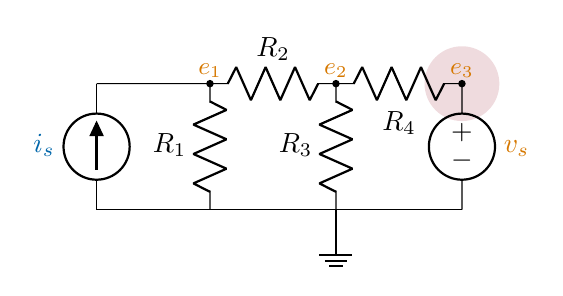
\begin{tikzpicture}[scale=0.8]
        \only<4->{\node[halo] at (5.8,2) {};}
        \exA{1}
      \end{tikzpicture}\\[6pt]
      Unknowns $\e{1}$, $\e{2}$, $\e{3}$: three equations needed.
    \end{column}
    \begin{column}{0.52\textwidth}
      \small
      \onslide<2->{%
      \textbf{Node 1:} \
      $\displaystyle -\Icol{i_s} + \frac{\e{1}}{R_1} + \frac{\e{1} - \e{2}}{R_2} = 0$\\[8pt]
      \textbf{Node 2:} \
      $\displaystyle \frac{\e{2} - \e{1}}{R_2} + \frac{\e{2}}{R_3} + \frac{\e{2} - \e{3}}{R_4} = 0$\\[12pt]}
      \onslide<3->{%
      \textbf{Question.} What does KCL at node 3 give?\\[8pt]}
      \onslide<4->{%
      The current through $\Vcol{v_s}$ is unknown: KCL gives \alert{no useful equation} in
      $\e{1}$, $\e{2}$, $\e{3}$.\\[8pt]}
      \onslide<5->{%
      But $\e{3} = \Vcol{v_s}$: this is the third equation.}
    \end{column}
  \end{columns}
\end{frame}

%--------------------------------------------------------------
\begin{frame}{A voltage source to the ground}
  \vfill
  \begin{block}{Remark}
    If an independent voltage source $\Vcol{v_s}$ is connected between the ground and node $k$,
    then $\e{k} = \Vcol{v_s}$ is \alert{known}.\\[4pt]
    So $\e{k}$ is \alert{not} an unknown, and we do not write KCL at node $k$.
  \end{block}
  \vfill
  \begin{center}
    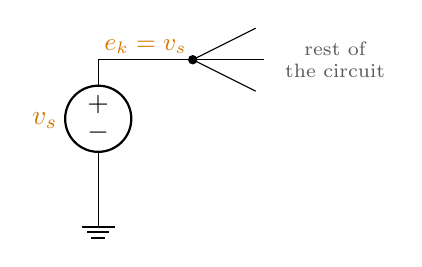
\begin{tikzpicture}
      \draw (0,0) node[ground] {} -- (0,0.2) to[american voltage source, invert, l=$\Vcol{v_s}$] (0,1.7) -- (1.2,1.7);
      \nodev{1.2,1.7}{above left}{$e_k = v_s$}
      \draw (1.2,1.7) -- (2.0,2.1); \draw (1.2,1.7) -- (2.1,1.7); \draw (1.2,1.7) -- (2.0,1.3);
      \node[capn, anchor=west] at (2.25,1.7) {rest of\\the circuit};
    \end{tikzpicture}
  \end{center}
  \vfill
\end{frame}

%--------------------------------------------------------------
\begin{frame}{Example 11.2, revisited}
  \begin{columns}[c,onlytextwidth]
    \begin{column}{0.46\textwidth}
      \centering
      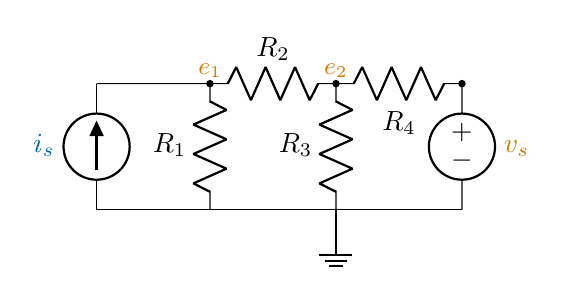
\begin{tikzpicture}[scale=0.8]
        \exA{2}
      \end{tikzpicture}\\[6pt]
      Unknowns $\e{1}$, $\e{2}$ only: two equations needed.
    \end{column}
    \begin{column}{0.52\textwidth}
      \small
      \textbf{Node 1:} \
      $\displaystyle -\Icol{i_s} + \frac{\e{1}}{R_1} + \frac{\e{1} - \e{2}}{R_2} = 0$\\[8pt]
      \textbf{Node 2:} \
      $\displaystyle \frac{\e{2} - \e{1}}{R_2} + \frac{\e{2}}{R_3} + \frac{\e{2} - \Vcol{v_s}}{R_4} = 0$\\[12pt]
      \onslide<2->{%
      $\begin{bmatrix}
        \frac{1}{R_1} + \frac{1}{R_2} & -\frac{1}{R_2}\\[3pt]
        -\frac{1}{R_2} & \frac{1}{R_2} + \frac{1}{R_3} + \frac{1}{R_4}
      \end{bmatrix}
      \begin{bmatrix} \e{1}\\[3pt] \e{2} \end{bmatrix}
      =
      \begin{bmatrix} \Icol{i_s}\\[3pt] \Vcol{v_s}/R_4 \end{bmatrix}$\\[10pt]}
      \onslide<3->{%
      The known $\Vcol{v_s}$ moves to the right side.\\[3pt]
      $\Vcol{v_s}/R_4$ acts like a current source into node 2: a source transformation.}
    \end{column}
  \end{columns}
\end{frame}

%==============================================================
\roadmapframe{4}

%--------------------------------------------------------------
\begin{frame}{Example 11.3: a voltage source between two nodes}
  \vfill
  \begin{center}
    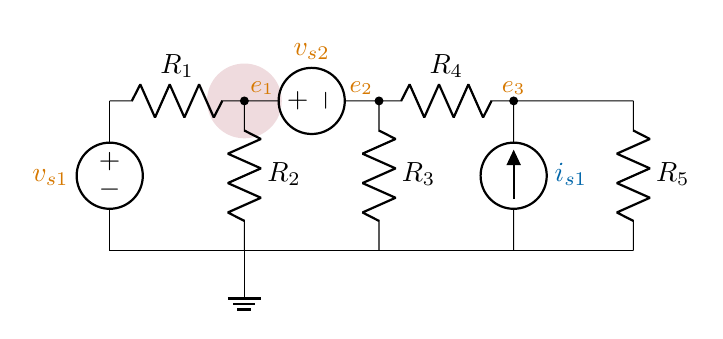
\begin{tikzpicture}[scale=0.95]
      \only<1-2>{\node[halo] at (1.8,2) {};}
      \exB{0}
    \end{tikzpicture}
  \end{center}
  \vfill
  \begin{itemize}\itemsep6pt
    \item \textbf{Question.} Write KCL at node 1: what is the current through $\Vcol{v_{s2}}$?
    \item<2-> It \alert{cannot} be written with $\e{1}$ and $\e{2}$: the law of a voltage source
      fixes its voltage, not its current.
    \item<3-> \textbf{Modified node voltage analysis} offers two ways out:
      \alert{Method I} (its current is a new unknown) and \alert{Method II} (a supernode).
  \end{itemize}
  \vfill
\end{frame}

%--------------------------------------------------------------
\begin{frame}{Method I: the current as an unknown}
  \begin{center}
    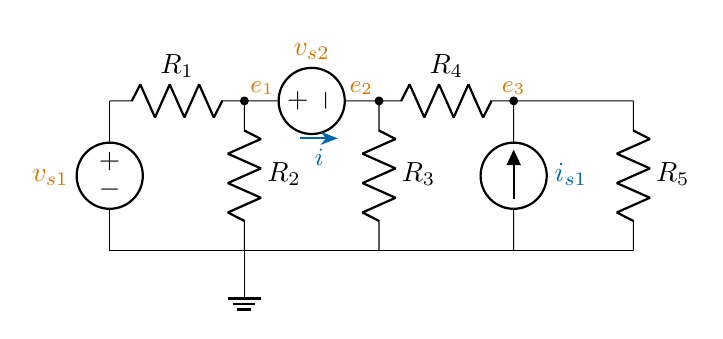
\begin{tikzpicture}[scale=0.95]
      \exB{1}
    \end{tikzpicture}
  \end{center}
  \vspace{-4pt}
  \begin{columns}[t,onlytextwidth]
    \begin{column}{0.53\textwidth}
      \small
      \textbf{Node 1:} \
      $\displaystyle \frac{\e{1} - \Vcol{v_{s1}}}{R_1} + \frac{\e{1}}{R_2} + \Icol{i} = 0$\\[5pt]
      \onslide<2->{%
      \textbf{Node 2:} \
      $\displaystyle -\Icol{i} + \frac{\e{2}}{R_3} + \frac{\e{2} - \e{3}}{R_4} = 0$\\[5pt]}
      \onslide<3->{%
      \textbf{Node 3:} \
      $\displaystyle \frac{\e{3} - \e{2}}{R_4} - \Icol{i_{s1}} + \frac{\e{3}}{R_5} = 0$}
    \end{column}
    \begin{column}{0.44\textwidth}
      \small
      Unknowns: $\e{1}$, $\e{2}$, $\e{3}$ and the current $\Icol{i}$.\\[8pt]
      \onslide<4->{%
      Four unknowns, three equations: one more is needed.\\[8pt]}
      \onslide<5->{%
      \textbf{Constraint:} \ $\e{1} - \e{2} = \Vcol{v_{s2}}$, the law of the source.}
    \end{column}
  \end{columns}
\end{frame}

%--------------------------------------------------------------
\begin{frame}{Method I: matrix form}
  \vfill
  \[
    \begin{bmatrix}
      G_1 + G_2 & 0 & 0 & 1\\
      0 & G_3 + G_4 & -G_4 & -1\\
      0 & -G_4 & G_4 + G_5 & 0\\
      1 & -1 & 0 & 0
    \end{bmatrix}
    \begin{bmatrix} \e{1}\\ \e{2}\\ \e{3}\\ \Icol{i} \end{bmatrix}
    =
    \begin{bmatrix} G_1\Vcol{v_{s1}}\\ 0\\ \Icol{i_{s1}}\\ \Vcol{v_{s2}} \end{bmatrix},
    \qquad G_k = \frac{1}{R_k}
  \]
  \vfill
  \begin{itemize}\itemsep7pt
    \item<2-> The first three rows are KCL; the last row is the constraint.
    \item<3-> The unknown current $\Icol{i}$ is part of the solution: we get it directly.
    \item<4-> The price: one more unknown and one more equation.
  \end{itemize}
  \vfill
\end{frame}

%==============================================================
\roadmapframe{5}

%--------------------------------------------------------------
\begin{frame}{Method II: the supernode}
  \begin{center}
    \begin{tikzpicture}[scale=0.95]
      \only<1-2>{\exB{1}}%
      \only<3->{\exB{2}}%
    \end{tikzpicture}
  \end{center}
  \vspace{-4pt}
  \begin{columns}[t,onlytextwidth]
    \begin{column}{0.5\textwidth}
      \textbf{Question.} Can we get rid of the unknown $\Icol{i}$?\\[8pt]
      \onslide<2->{%
      Add the KCL equations of nodes 1 and 2.\\[3pt]
      $\Icol{i}$ leaves node 1 and enters node 2, so it \alert{cancels}.}
    \end{column}
    \begin{column}{0.47\textwidth}
      \onslide<3->{%
      This is KCL for a closed surface around both nodes and the source.\\[6pt]}
      \onslide<4->{%
      \begin{block}{Supernode}
        Write KCL as if the two nodes of the voltage source were a single node.
      \end{block}}
    \end{column}
  \end{columns}
\end{frame}

%--------------------------------------------------------------
\begin{frame}{Method II: the equations}
  \begin{center}
    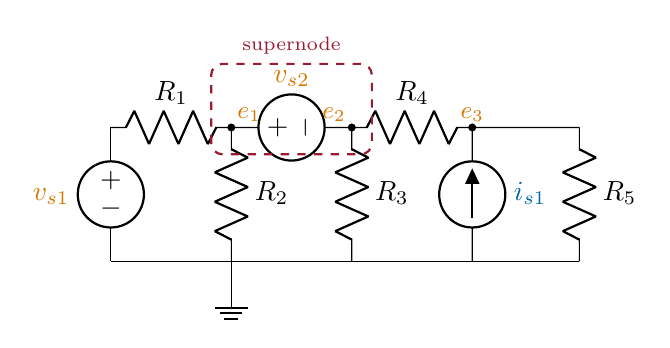
\begin{tikzpicture}[scale=0.85]
      \exB{2}
    \end{tikzpicture}
  \end{center}
  \vspace{-10pt}
  \begin{columns}[t,onlytextwidth]
    \begin{column}{0.49\textwidth}
      \small
      \textcolor{metured}{\textbf{Supernode:}} \
      $\displaystyle \frac{\e{1} - \Vcol{v_{s1}}}{R_1} + \frac{\e{1}}{R_2} + \frac{\e{2}}{R_3}
        + \frac{\e{2} - \e{3}}{R_4} = 0$\\[4pt]
      \textbf{Node 3:} \
      $\displaystyle \frac{\e{3} - \e{2}}{R_4} - \Icol{i_{s1}} + \frac{\e{3}}{R_5} = 0$\\[4pt]
      \textbf{Constraint:} \ $\e{1} - \e{2} = \Vcol{v_{s2}}$
    \end{column}
    \begin{column}{0.49\textwidth}
      \small
      \onslide<2->{%
      \footnotesize
      \[
      \begin{bmatrix}
        G_1 + G_2 & G_3 + G_4 & -G_4\\
        0 & -G_4 & G_4 + G_5\\
        1 & -1 & 0
      \end{bmatrix}
      \begin{bmatrix} \e{1}\\ \e{2}\\ \e{3} \end{bmatrix}
      =
      \begin{bmatrix} G_1\Vcol{v_{s1}}\\ \Icol{i_{s1}}\\ \Vcol{v_{s2}} \end{bmatrix}
      \]\small}
      \onslide<3->{%
      Three unknowns, three equations.\\[2pt]
      The matrix is \alert{not} symmetric any more.}
    \end{column}
  \end{columns}
\end{frame}

%--------------------------------------------------------------
\begin{frame}{Method I or Method II?}
  \vfill
  \begin{center}
  \renewcommand{\arraystretch}{1.4}
  \begin{tabular}{@{}l l l@{}}
  \toprule
   & \textbf{Method I} & \textbf{Method II}\\
  \midrule
  extra unknown & the current $\Icol{i}$ of the source & none\\
  KCL & at every non-ground node & at the supernode, and the others\\
  extra equation & the constraint $\e{1} - \e{2} = \Vcol{v_{s2}}$ & the same constraint\\
  size (this example) & $4 \times 4$ & $3 \times 3$\\
  the current $\Icol{i}$ & part of the solution & from KCL afterwards\\
  \bottomrule
  \end{tabular}
  \end{center}
  \vfill
  \onslide<2->{\begin{center}
    Both give the same node voltages.\\[3pt]
    The constraint is always the law of the voltage source.
  \end{center}}
  \vfill
\end{frame}

%==============================================================
\roadmapframe{6}

%--------------------------------------------------------------
\begin{frame}{Example 11.4: a dependent source}
  \begin{columns}[c,onlytextwidth]
    \begin{column}{0.47\textwidth}
      \centering
      \begin{tikzpicture}[scale=1.0]
        \only<1-2>{\exC{0}}%
        \only<3->{\exC{1}}%
      \end{tikzpicture}
    \end{column}
    \begin{column}{0.52\textwidth}
      \textbf{Question.} Find the power absorbed by the $3\ohm$ resistor.\\[10pt]
      \onslide<2->{%
      The voltage source $\Vcol{v_x}$ is between nodes 3 and 2; neither is the ground.\\[8pt]}
      \onslide<3->{%
      So use a supernode \nd{S} around nodes 2 and 3.\\[8pt]}
      \onslide<4->{%
      Unknowns: $\e{1}$, $\e{2}$, $\e{3}$.\\[3pt]
      Equations: KCL at node 1, KCL at \nd{S}, and a constraint.}
    \end{column}
  \end{columns}
\end{frame}

%--------------------------------------------------------------
\begin{frame}{Example 11.4: the equations}
  \begin{columns}[c,onlytextwidth]
    \begin{column}{0.44\textwidth}
      \centering
      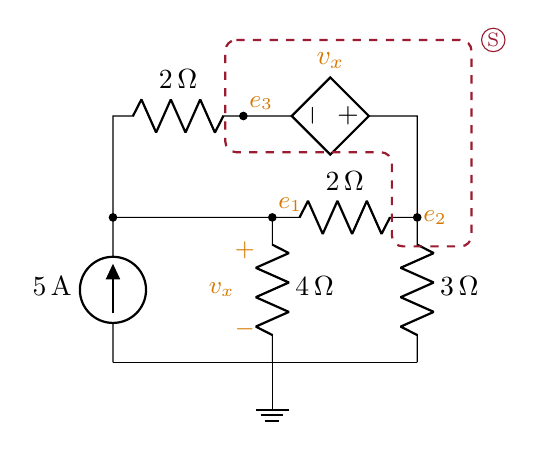
\begin{tikzpicture}[scale=0.92]
        \exC{1}
      \end{tikzpicture}
    \end{column}
    \begin{column}{0.54\textwidth}
      \small
      \textbf{Node 1:} \
      $\displaystyle -5 + \frac{\e{1} - \e{3}}{2} + \frac{\e{1}}{4} + \frac{\e{1} - \e{2}}{2} = 0
      \ \ (1)$\\[8pt]
      \onslide<2->{%
      \textbf{Supernode \nd{S}:} \
      $\displaystyle \frac{\e{3} - \e{1}}{2} + \frac{\e{2} - \e{1}}{2} + \frac{\e{2}}{3} = 0
      \ \ (2)$\\[10pt]}
      \onslide<3->{%
      \textbf{Question.} What is the constraint?\\[6pt]}
      \onslide<4->{%
      The source: $\e{2} - \e{3} = \Vcol{v_x}$.\\[4pt]}
      \onslide<5->{%
      Its control: $\Vcol{v_x} = \e{1}$, the voltage of the $4\ohm$.\\[6pt]}
      \onslide<6->{%
      \textbf{Constraint:} \ $\e{2} - \e{3} = \e{1} \quad (3)$\\[6pt]
      Three equations, three unknowns.}
    \end{column}
  \end{columns}
\end{frame}

%--------------------------------------------------------------
\begin{frame}{Example 11.4: solve}
  \vfill
  \begin{itemize}\itemsep8pt
    \item (1): \ $\tfrac{5}{4}\e{1} - \tfrac12\e{2} - \tfrac12\e{3} = 5$; \ put
      $\e{1} = \e{2} - \e{3}$ from (3): \quad
      $\tfrac34\e{2} - \tfrac74\e{3} = 5 \quad (4)$
    \item<2-> (2): \ $-\e{1} + \tfrac56\e{2} + \tfrac12\e{3} = 0$; \ put (3): \quad
      $-\tfrac16\e{2} + \tfrac32\e{3} = 0 \ \Rightarrow\ \e{3} = \tfrac19\e{2} \quad (5)$
    \item<3-> (4) and (5): \ $\tfrac34\e{2} - \tfrac{7}{36}\e{2} = \tfrac{20}{36}\e{2} = 5$
      \quad$\Rightarrow$\quad $\e{2} = 9\V$
    \item<4-> Then $\e{3} = 1\V$ and $\e{1} = \e{2} - \e{3} = 8\V$.
  \end{itemize}
  \vfill
  \onslide<5->{%
  \begin{center}
    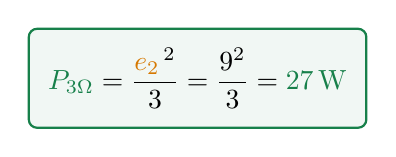
\begin{tikzpicture}
      \node[draw=cpow, thick, fill=cpow!6, rounded corners=3pt, inner sep=7pt]
        {$\displaystyle \Pcol{P_{3\Omega}} = \frac{\e{2}^{\,2}}{3} = \frac{9^2}{3} = \Pcol{27\W}$};
    \end{tikzpicture}
  \end{center}}
  \vfill
\end{frame}

%--------------------------------------------------------------
\begin{frame}{Dependent sources}
  \vfill
  \begin{itemize}\itemsep10pt
    \item A dependent source is handled like an independent one of the same kind.
    \item<2-> Its control variable ($\Vcol{v_x}$ here) is written with node voltages: this
      gives the \alert{constraint equation}.
  \end{itemize}
  \vfill
  \onslide<3->{%
  \begin{block}{Remark}
    If a dependent voltage source is connected between node $k$ and the ground, do
    \alert{not} write KCL at node $k$: its current is not known.\\[4pt]
    Write the constraint that the dependent source gives instead.
  \end{block}}
  \vfill
\end{frame}

%--------------------------------------------------------------
\roadmapframe{7}

%--------------------------------------------------------------
\begin{frame}{Exercise: choose node 3 as the ground}
  \begin{columns}[c,onlytextwidth]
    \begin{column}{0.44\textwidth}
      \centering
      \begin{tikzpicture}[scale=0.95]
        \only<1>{\exC{0}}%
        \only<2->{\exC{2}}%
      \end{tikzpicture}
    \end{column}
    \begin{column}{0.54\textwidth}
      \small
      \textbf{Question.} Redo the example with node 3 as the ground. Does the answer
      change?\\[8pt]
      \onslide<2->{%
      Now $\Vcol{v_x}$ is between node 2 and the ground: no supernode is needed.\\[6pt]}
      \onslide<3->{%
      Unknowns: $\ep{1}$, $\ep{2}$ and $\ep{0}$, the old ground.\\[8pt]}
      \onslide<4->{%
      \textbf{Node 1:} \
      $\displaystyle -5 + \frac{\ep{1}}{2} + \frac{\ep{1} - \ep{0}}{4} + \frac{\ep{1} - \ep{2}}{2} = 0$\\[5pt]
      \textbf{Node 0:} \
      $\displaystyle 5 + \frac{\ep{0} - \ep{1}}{4} + \frac{\ep{0} - \ep{2}}{3} = 0$\\[5pt]}
      \onslide<5->{%
      \textbf{Constraint:} \ $\ep{2} = \Vcol{v_x} = \ep{1} - \ep{0}$; \ no KCL at node 2.}
    \end{column}
  \end{columns}
\end{frame}

%--------------------------------------------------------------
\begin{frame}{Exercise: the solution}
  \vfill
  \begin{itemize}\itemsep8pt
    \item Put the constraint into both KCL equations:
      \[
        3\ep{1} + \ep{0} = 20, \qquad -7\ep{1} + 11\ep{0} = -60 .
      \]
    \item<2-> So $\ep{1} = 7\V$, \ $\ep{0} = -1\V$, \ $\ep{2} = 8\V$.
    \item<3-> The $3\ohm$ is between nodes 2 and 0:
      $\Pcol{P_{3\Omega}} = \dfrac{(\ep{2} - \ep{0})^2}{3} = \dfrac{9^2}{3} = \Pcol{27\W}$,
      \alert{the same}.
  \end{itemize}
  \vfill
  \onslide<4->{%
  \begin{center}
    Every node voltage drops by the same $\e{3} = 1\V$: \ $8 \to 7$, \ $9 \to 8$, \ $0 \to -1$.\\[5pt]
    The branch voltages, so the currents and the powers, do not change.
  \end{center}}
  \vfill
  \onslide<5->{%
  \begin{center}
    \alert{Tip:} put the ground at one end of a voltage source; this saves a supernode.
  \end{center}}
  \vfill
\end{frame}

%--------------------------------------------------------------
\begin{frame}{Summary}
  \vfill
  \begin{center}
  \renewcommand{\arraystretch}{1.45}
  \small
  \begin{tabular}{@{}>{\raggedright}p{4.1cm} >{\raggedright\arraybackslash}p{8.6cm}@{}}
  \toprule
  \textbf{In the circuit} & \textbf{What to do}\\
  \midrule
  resistors and current sources & KCL at every non-ground node: $Y_n\Vcol{\mathbf{e}} = \Icol{\mathbf{i}_s}$, by inspection; $Y_n$ is symmetric\\
  a voltage source from the ground to node $k$ & $\e{k} = \Vcol{v_s}$ is known; no KCL at node $k$\\
  a voltage source between two nodes & Method I: its current as an unknown, plus the constraint\newline
    Method II: KCL at the supernode, plus the constraint\\
  a dependent source & write its control variable with node voltages: a constraint\\
  the choice of ground & any node; the branch voltages and currents do not change\\
  \bottomrule
  \end{tabular}
  \end{center}
  \vfill
  \begin{center}
    After the node voltages: $\Vcol{\mathbf{v}} = A^T\Vcol{\mathbf{e}}$, then the currents from the element laws.
  \end{center}
  \vfill
\end{frame}

\end{document}
